\chapter{NOOSFERO}

O Noosfero é uma plataforma \textit{open source} para a construção de redes sociais
e colaborativas. Desenvolvido em Ruby on Rails e licenciado sob AGPL versão 3, o
projeto ainda conta com desenvolvimento ativo.

Além dos mecanismos de interação social, o Noosfero também conta com um sistema de
gerenciamento de conteúdo, o que possibilita a criação de \textit{blogs} e o
compartilhamento de arquivos. A plataforma também pode ser estendida por
\textit{plugins} desenvolvidos pela comunidade, e conta com o conceito de
\textit{environments}, que permitem a criação de diversas redes isoladas funcionando
sobre uma mesma instância da aplicação.

\begin{figure}[h]
	\centering
		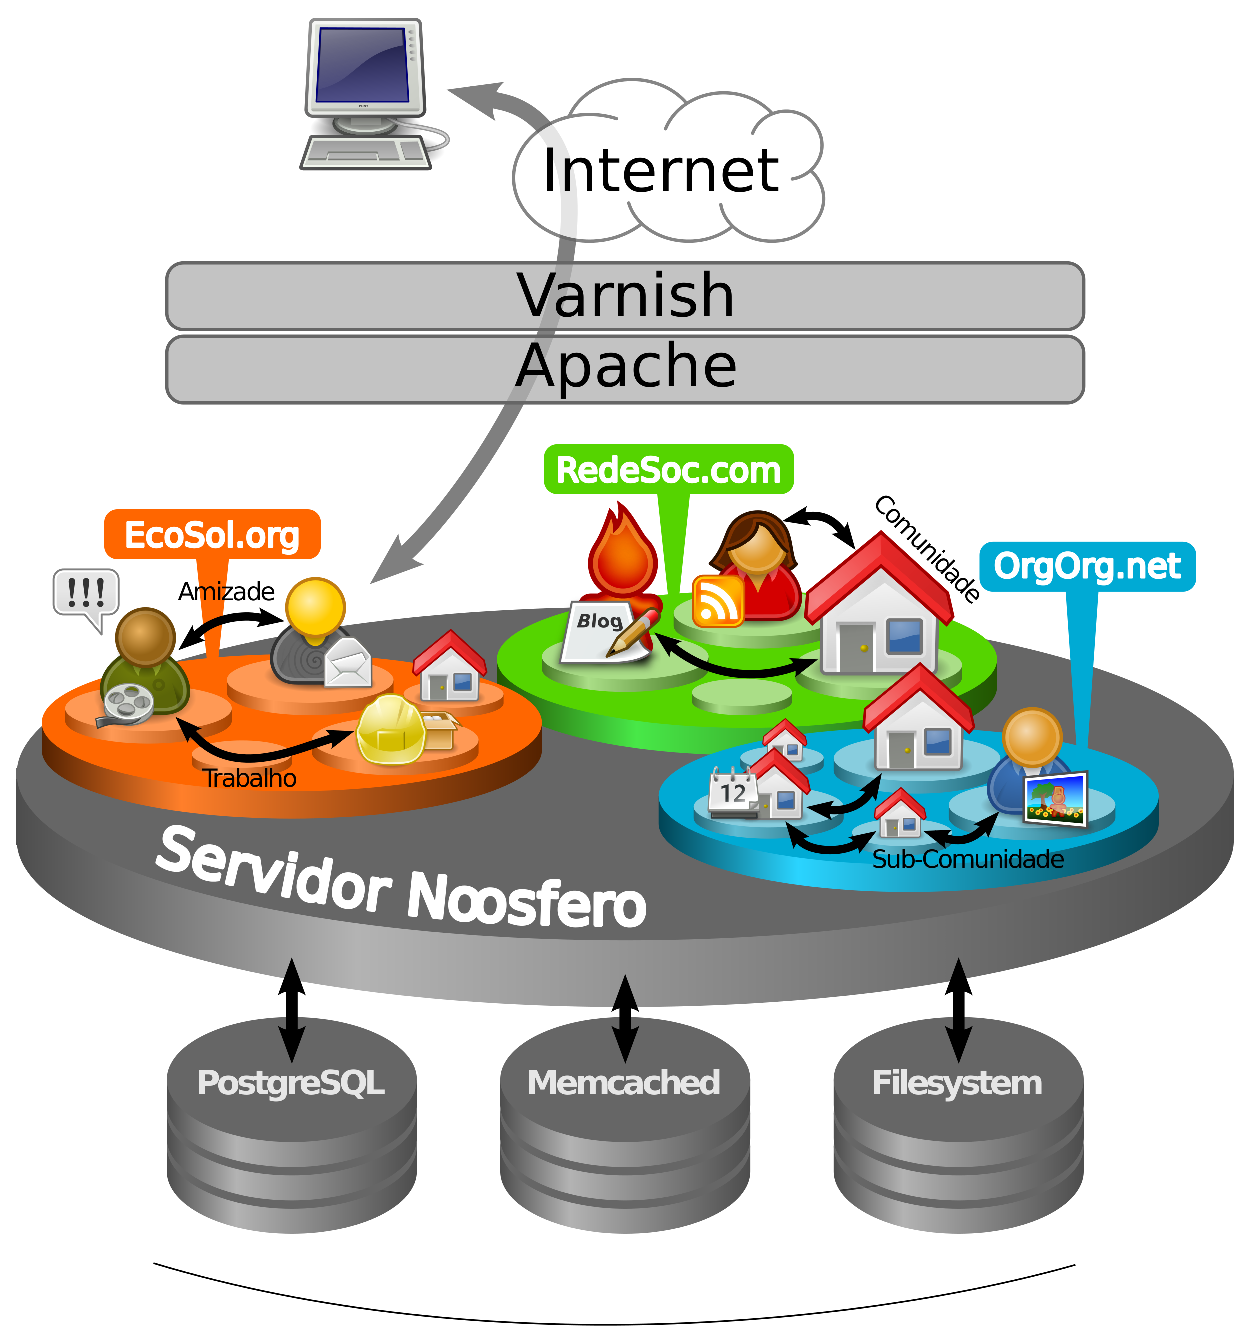
\includegraphics[keepaspectratio=true,scale=0.4]{figuras/noosfero_estrutura.eps}
	\caption{Arquitetura do Noosfero}
	\label{fig:noosferoEstrutura}
\end{figure}
% adicionar fonte

As informações e publicações de pessoas e organizações podem ser públicas ou
privadas. Já os relacionamentos entre estas entidades podem ser tanto simétricos
como assimétricos.

Enquanto um relacionamento simétrico depende da concordância de ambas as partes para
o compartilhamento das informações privadas (como por exemplo amizades ou
filiações), um relacionamento assimétrico depende apenas do interesse de uma das
entidades em acompanhar as informações públicas de algum perfil (como no caso da
funcionalidade de seguidores).



\section{SUPORTE À FEDERAÇÃO}

As definições da federação no Noosfero surgiram no contexto de desenvolvimento do
projeto do Portal do Software Público, como resultado de uma consultoria executada
pela Cooperativa de Tecnologias Livres \cite{colivre2016}. O produto foi um
relatório que define os objetivos e requisitos da implementação de federação na
plataforma Noosfero.

A proposta é que seja possível realizar a integração não só com outras instâncias do
Noosfero, como também com outras redes sociais. Desta forma, é necessário adotar
especificações que tenham o mínimo de aderência na comunidade, ao menos em outros
projetos que investem na implementação da federação entre redes sociais. Os
protocolos Diaspora e OStatus foram escolhidos observando projetos como o Hubzilla,
Friendica, e o próprio Diaspora.

É interessante que mesmo a integração entre redes Noosfero respeite os padrões
adotados pelos protocolos de referência, evitando a criação de outro padrão que não
reconhecido pelo restante dos projetos. No entanto, implementar a federação
respeitando os padrões existentes pode exigir uma refatoração da arquitetura ou das
funcionalidades da plataforma. Por exemplo, nenhum dos protocolos de referência
respeita o conceito de relacionamentos simétricos, padrão no Noosfero até então.


\subsection{Federação entre redes Noosfero}

As primeiras contribuições com a federação no Noosfero foram na integração de
instâncias diferentes da plataforma. As atividades foram definidas de acordo com
um \textit{roadmap} que dividiu a implementação em quatro fases, que cobrem desde
a reestruturação da arquitetura da aplicação, até a construção dos mecanismos
necessários para a autenticação e relação entre as redes.

O protocolo construído entre redes Noosfero é baseado nas especificações do
WebFinger e OAuth para a descoberta de identidade e autorização de perfis,
respectivamente. Em relação à comunicação entre as redes, o protocolo Diaspora foi
definido como referência. 

\subsubsection{Fase 1: preparação}

Até a versão 1.5 do Noosfero, todos os relacionamentos entre as entidades da rede
eram baseados no conceito de relacionamento simétrico. No entanto, a aderência

Na fase de preparação foram introduzidos os relacionamentos assimétricos através da
funcionalidade de seguidores. Seguidores podem visualizar as atividades e
informações públicas

\subsubsection{Fase 2: intercomunicações}

% WebFinger, ExternalX...
% Autenticação, comentários...
% Sugestão de artigos?

\subsubsection{Fase 3: integração externa}

% Evolução do oauth

\subsubsection{Fase 4: inter-relações}

% Relações entre usuários de diferentes redes


\subsection{Federação com outras redes sociais}

A implementação da federação com redes não Noosfero devem usar a infraestrutura
definida nas fases de desenvolvimento executadas, principalmente os mecanismos
de usuários externos e troca de mensagens.

Já que não existe um padrão para a federação de redes sociais, é interessante
seguir as especificações implementadas por outros projetos que também possuam
iniciativas de integração significativas, como o Hubzilla e o Diaspora, oferecendo
ao menos um nível limitado de suporte. A implementação do protocolo Diaspora deve
ser priorizada em relação ao OStatus, visto que não há mobilização na comunidade em
relação a este último.

% projeto
% o que a federação com outras redes deve cobrir
Requisitos:

\begin{itemize}
  \item{Autenticação...}
  \item{Whitelist...}
  \item{Inter relações...}
  \item{Notificações...}
  \item{Atualização do conteúdo...}
  \item{}
\end{itemize}

\subsubsection{Implementação do Protocolo Diaspora}



